\subsubsection{\textit{Kanban}}

O \textit{Kanban} é um método organizacional de desenvolvimento de software que permite a interação de várias áreas e membros do projeto por meio de cartões que contém o progresso de cada atividade. Cada cartão contém uma instrução a ser seguida pela área ou pelo integrante no qual foi designado para a atividade. Sendo assim, seu principal foco e fornecer um trabalho progressivo, apresentando as evoluções e dificuldades de forma clara e transparente, favorecendo uma cultura de melhoria contínua \cite{KANBAN2014}.

Portanto, a ferramenta \textit{Kanban} tem um grande potencial em trabalho conjunto para a finalização de um item em específico, justamente para que não ocorra nenhum gargalo na entrega de um item essencial para o trabalho do integrante ou da área seguinte. Outra grande característica é evitar ou diminuir o índice de trabalhos repetitivos que, por um eventual descuido, possa acontecer de desenvolvedores realizarem a mesma codificação de uma mesma função ou \textit{API - Application Programming Interface} (Interface de Programação de Aplicações), por exemplo.

A abordagem \textit{Kanban} foi criada pelo vice presidente da \textit{Toyota Motor Company}, o Sr. Taiichi Ohno, no qual teve como principal objetivo o aumento do valor agregado entregue nas atividades de cada colaborador de sua equipe. Com este pensamento,  Ohno concluiu que as pilhas de materiais estocados e as filas de espera eram equivalentes à um “dinheiro parado” que a empresa \textit{Toyota} estava desperdiçando. Portando,   Ohno uniu os princípios do método \textit{just in time} (determina que tudo deve ser feito na hora exata)  juntamente com o \textit{Jidoka} (determina que corrigir o problema em si não é o bastante, e sim corrigir a origem do problema) para elaborar um método mais aprimorado de organização dentro da empresa \textit{Toyota}, denominado \textit{Kanban} \cite{TOYOTA1977}.

Devido à sua simplicidade, fácil implantação, entendimento e manipulação, atualmente a abordagem \textit{Kanban} é utilizada em diversas empresas para realizar o controle de desempenho de diversas área. A \autoref{fig_kanban} está demonstrando um exemplo clássico de uma abordagem \textit{Kanban}.

\begin{figure}[h]
	\caption{\label{fig_kanban}Exemplo de uma abordagem \textit{Kanban}.}
	\begin{center}
		\resizebox{1\linewidth}{!}{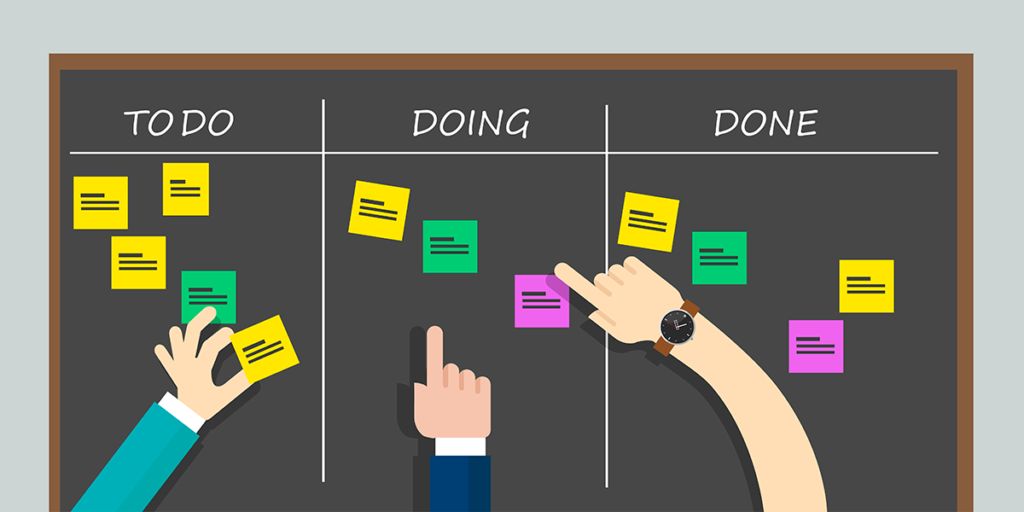
\includegraphics{4-Conteudo-Bibliografico/3-Engenharia-Software/kanban.png}}
	\end{center}
	\centering \legend{Disponível em: https://novida.com.br/blog/kanban/}
\end{figure}